\chapter{Bayesian Hyper-Heuristic}
\label{chap:bhh}

\begin{quote}
      \textit{
            ``The result is a posterior distribution which the agent may use as its new prior in the next step.'' - Pedro Domingos, The Master Algorithm: How the Quest for the Ultimate Learning Machine Will Remake Our World.
      }
\end{quote}

The above quote was the inspiration for the development of a novel \ac{HH} that uses \index{Bayesian}\textit{Bayesian} probability concepts as a selection mechanism to drive the heuristic selection process. Thus far the reader was presented with all of the necessary background information on \acp{ANN} in Chapter \ref{chap:anns}, low-level \index{heuristic}heuristics/\index{Optimiser}optimisers in Chapter \ref{chap:heuristics}, \acp{HH} in Chapter \ref{chap:hhs}  and lastly, \index{probability theory}probability theory in Chapter \ref{chap:probability}. These elements form the fundamental components that make up the proposed \Ac{BHH}. A detailed specification on the \Ac{BHH} can now be formulated. This chapter provides the detail around the theory, concept and implementation of the \Ac{BHH} and explains how it used to train \acp{ANN}. It is shown throughout this chapter that the \Ac{BHH} implements a probabilistic optimisation technique that implements and biases a \index{Gaussian Process}\textit{Gaussian process} towards good optimisation and performance. The remainder of the chapter is structured as follows:

\begin{itemize}
      \item \textbf{Section \ref{sec:bhh:overview}} provides a brief overview of the \Ac{BHH} optimiser.

      \item \textbf{Section \ref{sec:bhh:architecture}} presents the general architecture, \Ac{HH} framework and the various components that make up the \index{Optimiser}optimiser.

      \item \textbf{Section \ref{sec:bhh:heuristic_pool}} discusses the collection of low-level \index{heuristic}heuristics, referred to as the \index{heuristic}\textit{heuristic pool} and puts emphasis on the importance of a diverse set of low-level \index{heuristic}heuristics.

      \item \textbf{Section \ref{sec:bhh:entity_pool}} discusses the detail of the \index{Population}population and its \index{entity}entities, with specific detail provided on entity (local) and population (global) state and memory.

      \item \textbf{Section \ref{sec:bhh:initialisation_step}} presents the initialisation strategy in detail.

      \item \textbf{Section \ref{sec:bhh:selection_mechanism}} presents the \index{Bayesian}\textit{Bayesian} probabilistic model that is used as a selection mechanism.

      \item \textbf{Section \ref{sec:bhh:heuristic_entity_selections}} discusses heuristic-entity selections and how these two concepts are utilised together.

      \item \textbf{Section\ref{sec:bhh:model}} discusses the models that can be optimised using the \Ac{BHH}, specifically referring to its application to training \acp{FFNN}.

      \item \textbf{Section \ref{sec:bhh:train_test_datasets}} briefly discussed the role of the train and test datasets during training.

      \item \textbf{Section \ref{sec:bhh:loss_function}} discusses model evaluation and the role of the loss/cost function.

      \item \textbf{Section \ref{sec:bhh:domain_barrier}} discusses the domain barrier that exists between the high-level \ac{BHH} and low-level heuristics in the \index{heuristic pool}heuristic pool.

      \item \textbf{Section \ref{sec:bhh:performance_log}} presents the performance log and discusses performance measurement in more detail.

      \item \textbf{Section \ref{sec:bhh:credit_assignment_strategy}} discussed credit assignment and move acceptance strategies in detail.

      \item \textbf{Section \ref{sec:bhh:optimisation_step}} presents the learning mechanisms by which the probabilistic model can be optimised.

      \item \textbf{Section \ref{sec:bhh:hyper_parameters}} summarises and discusses the associated \index{hyper-parameters}hyper-parameters and default values.

      \item The pseudo-code algorithm for the \ac{BHH} is given in \textbf{Section \ref{sec:bhh:algorithm}}.

      \item Finally, a summary of the chapter is provide in \textbf{Section \ref{sec:bhh:summary}}.
\end{itemize}


\section{Overview}
\label{sec:bhh:overview}

This section provides an overview of the workings of the \Ac{BHH}. To start the discussion, consider the following analogy:\\
\\
\textit{
      Bob is a teacher at a high school. Every year his students perform really well and he wins the prize for best teacher, evaluated by student performance. He is able to do this not just because he is a good teacher, but he understands that each student has a learning technique that works best for him/her. He exploits this concept by tailoring the teaching process to each students such that the result is an optimum mark for that student and by definition, the whole class. Bob knows that it is too timely to get to know each student, so he devises a model that does the allocations for him. This model uses a process of observation. With each evaluation opportunity he experiments by allocating different learning techniques to different students. He evaluates the student for the given opportunity and keeps a log of which learning technique he assigned to the student as well as the outcome. With each evaluation opportunity he updates his model by biasing the assignment process such that students generally get assigned learning techniques that yield the best performance for them.
}\\
\\
The key take-out from the analogy above is the concept that Bob can maximise student performance by updating his beliefs, over time, about which learning technique to assign to which (type of) student. He does this by biasing selection/assignment towards the best combinations of student, learning technique
and evaluation opportunity. This is the basic nature of the \Ac{BHH}. The students are analogous to a population of entities. The learning techniques are analogous to heuristics/optimisers. Evaluation opportunities are analogous to optimisation problems to be optimised. Student performance is analogous to optimisation capability and performance measurement. The general goal of the \ac{BHH} can be summarised as aiming to select and managing the appropriate  heuristic/optimiser and update step for each entity, at each optimisation step, while optimising some underlying model, which for this dissertation, is to train \acp{FFNN}.

Formal classification of the \Ac{BHH} is needed. Burke et al.~\cite{ref:burke:2010} proposed a classification mechanism that was discussed in detail in Chapter \ref{chap:hhs}. The same classification mechanism is used to classify the \ac{BHH}. For the first dimension of the classification, the authors propose that the \Ac{BHH} be classified as a \textit{selection} \ac{HH}. For the second dimension of the classification proposed, the authors propose that the \Ac{BHH} be classified as utilising \textit{perturbation} low-level heuristics. Furthermore, the \ac{BHH} is also classified as a population-based approach that includes meta-heuristics. Burke et al.~\cite{ref:burke:2010} further proposed the classification of \acp{HH} according to the source of the feedback used during learning. It can thus be said that the \ac{BHH} employs online learning according to this criteria, classifying it as an \textit{adaptive} \ac{HH}. A \textit{population-based, selection, meta-hyper-heuristic that utilised perturbation of low-level heuristics and online learning} seems like an mouthful, but technically, that is it's full and formal classification. A breakdown and motivation of these classifications is given below:

\begin{itemize}
      \item \textbf{Population-Based:} The \ac{BHH} follows a population-based approach where a number of different \index{candidate solution}candidate solutions, referred to as \index{entity}\textit{entities} work together to yield a global best solution. There is also the concept of a shared global state or memory.

      \item \textbf{Selection:} The \ac{BHH} implements a \index{heuristic}heuristic selection mechanism that selects from a collection of lower level \index{heuristic}heuristics' in a so-called \index{heuristic hool}\textit{heuristic pool}. There is also a measure of acceptance criteria through credit assignment strategies.

      \item \textbf{Meta:} Incorporates the classical/analytical gradient-based low level \index{heuristic}heuristics (typically from the \ac{ML} research space) as well as meta-heuristics such as other population-based \index{Meta-Heuristic}meta-heuristics (typically \ac{EC} research space).

      \item \textbf{Hyper-Heuristic:} There exists a domain barrier where the \ac{BHH} searches through the \textit{heuristic space} while lower level heuristics search through the \textit{solution space}.

      \item \textbf{Perturbation of Low-Level Heuristics:} Refers to the iterative optimisation approach followed by the \ac{BHH}. The \ac{BHH} considers a number of randomly initialised candidate solutions in the form of entities in a population. It is applied in an iterative manner, during the training process. It generally employs the two main processes of \acp{HH} with perturbation of heuristics. These include a \textit{selection step} that selects from low-level heuristics and applies them to entities/candidate solutions. It also includes an \textit{acceptance strategy}. The \ac{BHH} maintains entity and population state through update step operations that proxy update steps from different heuristics. More details on this concept is given later in Section \ref{sec:bhh:heuristic:proxies}.

      \item \textbf{Online Learning:} Refers to the source of the feedback used during training. The \ac{BHH} optimises, at a higher level, the selection and application of the \index{heuristic space}\textit{heuristic space} while low-level heuristics optimise entities' solution to the underlying model, in this case a \ac{FFNN}. This happens during training time, yielding the classification of utilising \textit{online} learning.
\end{itemize}

More detailed consideration of these elements are required. The following sections break down the \Ac{BHH} into its various parts, starting with a discussion on the high-level architecture next.


\index{Architecture}
\section{Architecture}
\label{sec:bhh:architecture}

This section aims to present the reader with all the high level components in the architecture of the \Ac{BHH}. Burke et al.~\cite{ref:burke:2010} proposed an initial framework for \acp{HH} and Grobler~\cite{ref:grobler:2015} further proposed a framework for a heterogeneous meta-\ac{HH}. These frameworks have been adapted for the implementation of the \Ac{BHH}. An illustration of the high-level architecture of the \Ac{BHH} is given in Figure \ref{fig:bhh_architecture} below.

\begin{figure}[H]
      \centering
      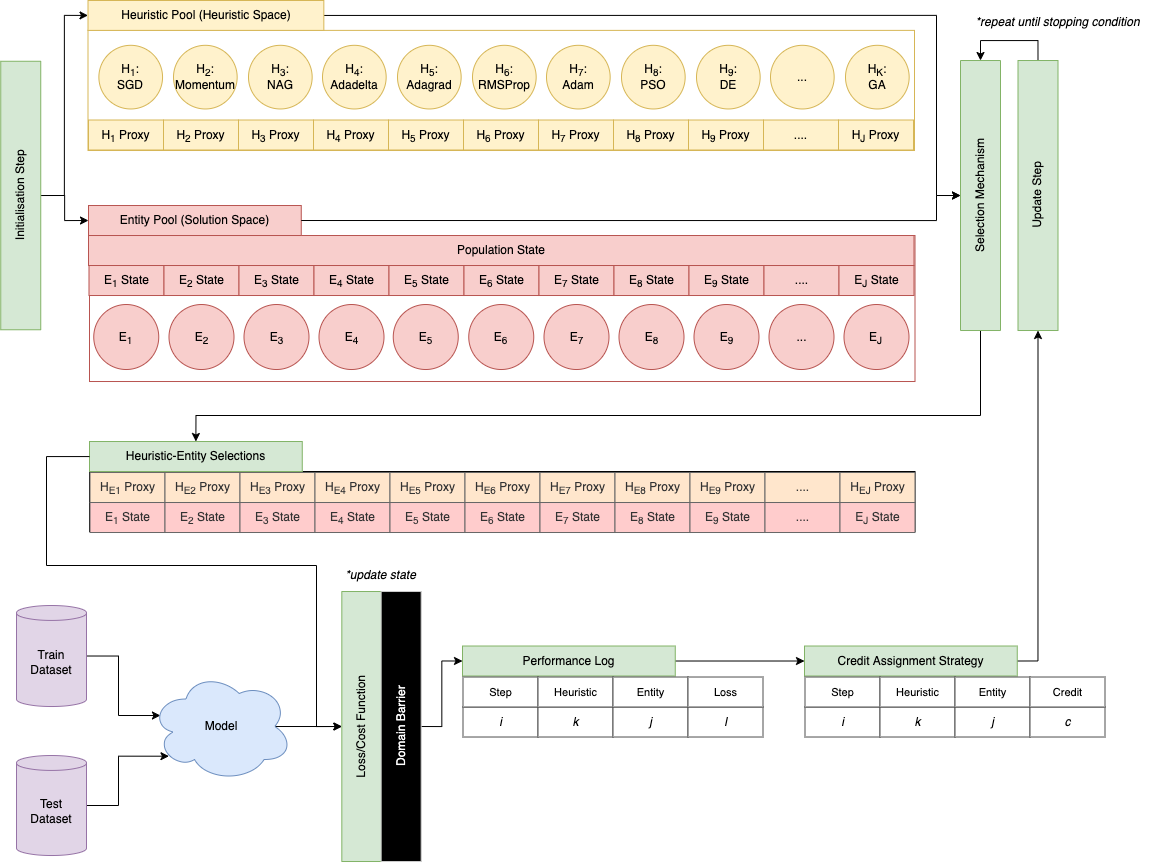
\includegraphics[width=1.0\textwidth]{bhh_architecture.png}
      \caption[The \index{Bayesian Hyper-Heuristics}Bayesian Hyper-Heuristic Architecture]{An illustration of
            the architecture and high level components of the \index{Bayesian Hyper-Heuristics}Bayesian Hyper-Heuristic.}
      \label{fig:bhh_architecture}
\end{figure}

At a high level, the architecture presented in Figure \ref{fig:bhh_architecture} above, presents the following main components:

\begin{itemize}
      \item \textbf{Heuristic Pool}: Contains a collection of low-level \index{heuristic}heuristics/\index{optimiser}optimisers. This is the \index{heuristic space}\textit{heuristic} space. Each heuristic has a proxy that is used to relay heuristic state update operations.

      \item \textbf{Entity Pool}: A collection of \index{entity}entities in a \index{population}population. These entities represent candidate solutions to the model. Each entity has its own state, but there is also a shared global population state.

      \item \textbf{Initialisation Step}: This is the execution of some initialisation strategy that determines how the entities in the entity pool (population) and the heuristics in the heuristic pool are initialised.

      \item \textbf{Selection Mechanism}: This is the implementation of the selection mechanism of selection \acp{HH}. In the case of the \ac{BHH}, the selection mechanism is a Bayesian probabilistic model.

      \item \textbf{Heuristic-Entity Selections}: This is the results of the selection mechanism. Heuristics are sampled/selected for each entity. Each entity's state will thus be manipulated by that particular heuristic's proxy methods.

      \item \textbf{Model}: The \index{model}model to be optimised. This forms the problem domain. In the case of this dissertation, the model is a \ac{FFNN}.Technically the model here simply refers to the architectural structure of the model, while entities represent that candidate solution (weights) to the model.

      \item \textbf{Train and Test Datasets}: The training set is used to train the model while the test set is used to evaluate the model's generalisation capabilities.

      \item \textbf{Loss/Cost Function}: The loss/cost function is the metric  by which the model is evaluated. In the case of supervised learning, the loss/cost function is a measure of distance between predicted output and the ground truth.

      \item \textbf{Domain Barrier}: A constraint on information flow, prohibiting high level components in the \index{heuristic space}\textit{heuristic} space from interacting and relaying information related to the \index{solution space}\textit{solution} space.

      \item \textbf{Performance Log}: Contains a record of heuristic-entity performance at each step of the training process.

      \item \textbf{Credit Assignment Strategy}: Implements a specific strategy to determine if the performance of an entity-heuristic combination is better than others or not.

      \item \textbf{Update Step}: The high level heuristic update step. This involves the mechanism by with the \ac{BHH} is optimised.
\end{itemize}

The above components are not described in enough detailed to properly illustrate their role in the \Ac{BHH}. To ensure proper clarity is given to each of these elements, a detailed discussion on each of these elements are presented next.


\index{Heuristic Pool}
\section{Heuristic Pool}
\label{sec:bhh:heuristic_pool}

This section discusses the concept of the heuristic pool, as implemented by the \ac{BHH}. Generally speaking, they heuristic pool is just a collection of low-level heuristics and make up the set of possible heuristics to select from. This is referred to as \text{heuristic space}. Importantly, since \acp{HH} optimise in heuristic space, it is from these lower-level heuristics that the \ac{BHH} must select and apply. The heuristic pool can then be defined in terms of size and/or heuristics that are included in the pool. These two aspects pose very important design choices. Both of these concepts can be empirically tested, however, one could argue the choice of design. Fundamentally, these design choices are about diversity. A brief discussion is given next on the trade-offs between exploration, exploitation and capability.

\index{Exploration}
\index{Exploitation}
\subsection{Diversity: Exploration, Exploitation and Capability}
\label{sec:bhh:heuristic_pool:diversity}

As with all \acp{HH}, the heuristics to be included in the heuristic pool is of great importance and should be carefully decided upon. A heuristic's eligibility for inclusion is determined by the following factors:

\begin{itemize}
      \item \textbf{Capability}: Certain heuristics are only capable of solving or optimising for certain problem types and domains. Examples include continuous vs. discrete, differentiable vs.  non-differentiable or static vs. dynamic problems.

      \item \textbf{Exploration and Exploitation Trade-off}: Some heuristics explore or exploit more than others. This could be due to the nature of the implementation or due to some hyper-parameter such as a learning rate.
\end{itemize}

An argument for diversity must thus be made. One of the benefits of \acp{HH} in general is that it will learn which heuristics to apply and when. The trade-off between exploration and exploitation should thus be outsourced to the \ac{BHH} itself. By including a diverse set of heuristics, based on the criteria mentioned above, the \ac{BHH} will learn to select and apply the appropriate heuristic at the appropriate time throughout the training process, naturally balancing a trade-off between exploration and exploitation. Heuristics that initially explore a lot should be selected when exploration is needed and heuristics that exploit a lot should be selected accordingly.

Notice however that diversity can not be achieved by simply including many different heuristics. The \ac{BHH} is still constraint by heuristic pool size. Consider that for every heuristic that is included, the demand for samples size required to learn with statistical certainty exponentially increases. Not only does a large heuristic pool drastically complicate the learning that is required by the \ac{BHH}, but it also drastically complicates the process of maintaining state. The next section provides the concept of heuristic update step proxies, an important component of the \ac{BHH}.

\index{Proxies}
\subsection{Proxies}
\label{sec:bhh:heuristic:proxies}

The concept of proxies arise from the sparsity of state as maintained by different heuristics. Since heuristics maintain different states, there is an uncertainty of state transition when switching between heuristics. Consider an example where the heuristic pool consists of just two heuristics. One heuristic is a gradient-based heuristic that maintains momentum such as \ac{Adam}. The other is a meta-heuristic that does not require a gradient at all such as \ac{PSO}. Both these heuristics track different parameters in their state. For \ac{Adam}, the expected gradient mean and variance is maintained, while the \ac{PSO} maintains record of the gbest and pbest solutions all of entities. A solution to this is to proxy heuristic state update operations. This allows us to maintain state in two parts:

\begin{itemize}
      \item \textbf{Primary State}: This refers to state the is originally maintained by a heuristic. The selected heuristic simply applies the normal state update operations to its state.

      \item \textbf{Proxied State}: This refers to state that is not directly maintained by the current selected heuristic, but can be updated by outsourcing the required state update operation to another heuristic.
\end{itemize}

Effectively this means that both primary and proxied state elements must be maintained together. Since entities represent candidate solutions, which are a form of state, entities are ideal components to store these state parameters. Thus, entities are extended to include the primary state elements of all the underlying low-level heuristics as well as the candidate solution (weights) for the model. At each heuristic-entity application step, all state elements per entity are updated either by primary method or by proxied method. The \ac{BHH} thus incorporates a state update operation proxy mapping as given in the example in Table \ref{tab:bhh:heuristic_pool:proxy_mapping_example} below.

\begin{table}[htbp]
      \centering
      \caption{State update operation proxy mapping example.}
      \label{tab:bhh:heuristic_pool:proxy_mapping_example}%
      \par\bigskip
      \resizebox{0.5\textwidth}{!}{
            \begin{tabular}{ccccc}
                                                                  &   & \multicolumn{3}{c}{State Parameter}                                                                                                                                                                                      \\
                  \cmidrule{3-5}                                  &   & 1                                                                      & 2                                                                      & 3                                                                      \\
                  \cmidrule{3-5}    \multirow{3}[1]{*}{Heuristic} & A & \cellcolor[rgb]{ .776,  .937,  .808}\textcolor[rgb]{ 0,  .38,  0}{n/a} & \cellcolor[rgb]{ 1,  .922,  .612}\textcolor[rgb]{ .612,  .341,  0}{B}  & \cellcolor[rgb]{ .776,  .937,  .808}\textcolor[rgb]{ 0,  .38,  0}{n/a} \\
                                                                  & B & \cellcolor[rgb]{ .776,  .937,  .808}\textcolor[rgb]{ 0,  .38,  0}{n/a} & \cellcolor[rgb]{ .776,  .937,  .808}\textcolor[rgb]{ 0,  .38,  0}{n/a} & \cellcolor[rgb]{ 1,  .922,  .612}\textcolor[rgb]{ .612,  .341,  0}{A}  \\
                                                                  & C & \cellcolor[rgb]{ .776,  .937,  .808}\textcolor[rgb]{ 0,  .38,  0}{n/a} & \cellcolor[rgb]{ 1,  .922,  .612}\textcolor[rgb]{ .612,  .341,  0}{B}  & \cellcolor[rgb]{ 1,  .922,  .612}\textcolor[rgb]{ .612,  .341,  0}{A}  \\
            \end{tabular}%
      }
\end{table}%

From the example given in Table \ref{tab:bhh:heuristic_pool:proxy_mapping_example}, when heuristic A is selected, it will outsource state update operations from heuristic B, for state parameter 2. Heuristic B will outsource from heuristic A, for state parameter 3. Finally, heuristic C will outsource from heuristic A and B, for state parameters 2 and 3 respectively. In this way, all heuristics maintain all the state parameters.

Notice however that this is a simple concept in principle, but requires detailed decomposition of the heuristics included in the heuristic pool.  Overlapping and unique state parameters must be identified so that a proxy mapping such as the one given in Table \ref{tab:bhh:heuristic_pool:proxy_mapping_example} can be constructed. A suggestion to simplify this process is to borrow concepts from the equations of motion from physics. These include \textit{position}, \textit{velocity}, \textit{acceleration} and \textit{momentum}. Expressing heuristic update steps according to these parameters drastically simplify the process. However, it is possible that heuristics implement unique state parameters that do not overlap, these have to be catered for in the proxy mapping.

These state parameters and update operations should not be considered in isolation. An example of this is position and velocity. Consider for example heuristics such as \acl{DE} and \aclp{GA}. These heuristics recombine entities. In this case, the concept of an equation of motion does not entirely make sense, since the displacement of its position is not a result of maintaining velocity or momentum, but rather by pure displacement through recombination. In this particular case, a solution to this is to apply the recombination operation to all secondary state parameters as well or to nullify secondary state parameters. Unfortunately there is no general solution and each heuristic must be carefully considered. The \ac{BHH} incorporates both of these approaches. The next section provides the reader with details around the entity pool.

\index{Entity Pool}
\section{Entity Pool}
\label{sec:bhh:entity_pool}

This section presents the details around the \index{entity pool}\textit{entity pool}. The \index{entity pool}entity pool refers to a collection of so-called individual \index{entity}\textit{entities}. A common naming convention for such a collection is a \textit{population} of entities. Similar to the heuristic pool that was described in Section \ref{sec:bhh:heuristic_pool} above, the entity pool size is an important design choice. The correct population size is thus a hyper-parameter that can be empirically evaluated.

The entity pool maintains two different types of state. These include entity (local) and population (global) state. Each of these are discussed in more detail next.

\index{Entity State}
\subsection{Entity State}
\label{sec:bhh:entity_pool:entity_state}

\index{entity}Entities represent \index{candidate solution}candidate solutions to the \index{model}model's trainable parameters (weights) and other heuristic-specific state parameters as was just discussed above in Section \ref{sec:bhh:heuristic:proxies}. It can be said that entities implement \textit{local} state. It was mentioned that these \index{entity}entities can be treated as physical \index{particle}\textit{particles} in a hyper-dimensional physical environment. This means that these \index{entity}entities model concepts from physics. For example, the candidate solution is represented as the \index{entity}entity's \textit{position} and an \index{entity}entity's velocity and acceleration, is analogous to the gradient and momentum of an \index{entity}entity respectfully. Examples of \index{Entity State}entity state parameters as derived from various low-level heuristics is given as follows:

\begin{itemize}
      \item \textbf{position}: General parameter that represents the actual candidate solution and is thus a primary state parameter for all heuristics.

      \item \textbf{velocity}: Directly implemented by heuristics such as \acp{PSO} can be derived proportionally from the gradient for gradient-based heuristics such as \ac{Momentum}.

      \item \textbf{gradient}: The last know gradient as derived from gradient-based heuristics.

      \item \textbf{position delta}: The last computed position delta between the current timestep and the previous timestep.

      \item \textbf{sum of the gradients squared}: As required and maintained by heuristics such as \ac{Adagrad}.

      \item \textbf{expected position delta variance}: As required and maintained by heuristics such as \ac{Adadelta}.

      \item \textbf{expected gradient mean}: As required and maintained by heuristics such as \ac{Momentum}, \ac{NAG} and \ac{Adam}.

      \item \textbf{expected gradient variance}: As required and maintained by heuristics such as \ac{RMSProp}, \ac{Adadelta} and \ac{Adam}.

      \item \textbf{personal best position}: Parameter that tracks that best known position by the entity thus far. As required and maintained by heuristics such as \ac{PSO}.

      \item \textbf{personal best loss}: Parameter that tracks that best known loss by the entity thus far. As required and maintained by heuristics such as \ac{PSO}.

      \item \textbf{loss}: General parameter that tracks the loss as achieved by the the entity throughout training.
\end{itemize}

From the list above it should become clear that entity state becomes increasingly complicated as the number of distinct heuristics included in the heuristic pool increases. Consider next the global state that is maintained.

\index{Population State}
\subsection{Population State}
\label{sec:bhh:entity_pool:population_state}


The \index{Population State}\textit{population state} refers to a collection of parameters that are shared between the \index{entity}entities in the population. This state is also referred to as \index{global state}\textit{global} state and represents the entity pool's memory of the population. The \index{population state}population state generally contains state parameters that are of importance to multiple heuristics and usually track the state of the population as a whole and not individual heuristic states. Some examples of population state that can arise from different heuristics is given below:

\begin{itemize}
      \item \textbf{\textit{entities}}: Naturally, the population state contains the list of entities in the population. List size determined by \index{Population Size}population size. Naturally this list contains multiple entities as with population based approaches such as \acp{PSO} and \acp{GA}.

      \item \textbf{\textit{ibest}} and \textbf{\textit{ibest loss}}: Refers to the best position and loss achieved by the population for the current iteration/step. This parameter is introduced by the \ac{BHH} itself through the requirements of the \textit{ibest} credit assignment strategy.

      \item \textbf{\textit{rbest}} and \textbf{\textit{rbest loss}}: Refers to the best position and loss achieved by the population for the current replay buffer/window size. This parameter is introduced by the \ac{BHH} itself through the requirements of the \textit{rbest} credit assignment strategy.

      \item \textbf{\textit{gbest}} and \textbf{\textit{gbest loss}}: Refers to the overall/global best position and loss achieved by the population for the entire training process. This parameter is introduced by heuristics such as \acp{PSO} and is also introduced by the \ac{BHH} itself through the requirements of the \textit{gbest} credit assignment strategy.
\end{itemize}

The reader was now introduced to both the heuristic pool and entity pool. The next section considers how the \ac{BHH} is initialised and makes specific reference to how these two pools of elements are initialised.

\section{Heuristic-Entity Selections}
\label{sec:bhh:heuristic_entity_selections}

The \ac{BHH} selects from the heuristic pool a low-level heuristic to be applied to an entity. The outcome of this selection process is a table that tracks which heuristic has been selected for which entity. The selection process is executed by the selection mechanism of the \ac{BHH} and is discussed later in Section \ref{sec:bhh:selection_mechanism}. These heuristic-entity combinations are applied to an underlying model. The next section provides clarity on the model component from the architecture of the \ac{BHH}.

\index{Model}
\section{Model}
\label{sec:bhh:model}

The \index{Model}model refers to the target \index{model}model to be optimised and is usually expressed as a complex mathematical function. For this dissertation, the authors focused specifically on shallow \acp{FFNN} (only one hidden layer). Figure \ref{fig:shallow_ffnn} below presents such a shallow \acp{FFNN}.

\begin{figure}[H]
      \centering
      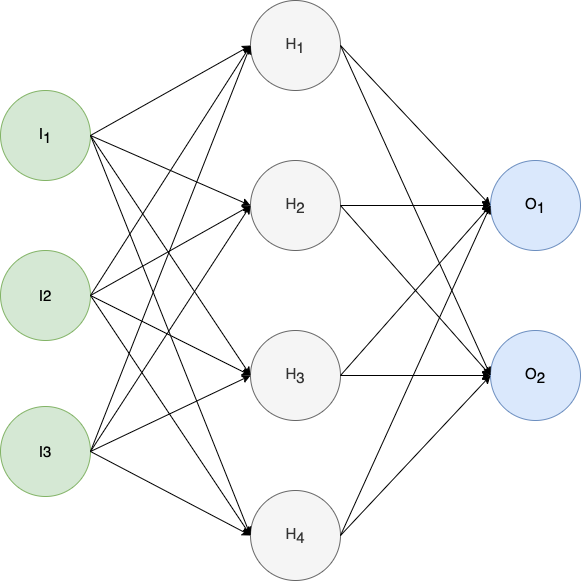
\includegraphics[width=0.4\textwidth]{shallow_ffnn.pdf}
      \caption[Shallow \index{Feedforward Neural Network}Feedforward Neural Network]{An illustration of
            a shallow \index{Feedforward Neural Network}Feedforward Neural Network.}
      \label{fig:shallow_ffnn}
\end{figure}

\section{Train and Test Datasets}
\label{sec:bhh:train_test_datasets}

The training of \ac{FFNN} is a supervised learning problem as was highlighted in Chapter \ref{chap:anns}. Therefore, the \ac{BHH} trains the model on training data from the training set, while is reserves an unseen set of test data in the test dataset for evaluation. It should be mentioned that the goal of the \ac{BHH} is to generalise well to the test set across a number of problem domains. As was previously mentioned, the test set should be sufficiently large to truly evaluate for generalisation capabilities. For the \ac{BHH}, it is proposed to have a 80-20\% split between the training and test set.

\section{Loss/Cost Function}
\label{sec:bhh:loss_function}

Chapter \ref{chap:anns} presented the concept of a loss/cost function that is used to evaluate the performance of \acp{ANN}. The \ac{BHH} uses this loss/cost function to evaluate the performance of a heuristic-entity combination. For classification problems, generally some entropy loss is used. For classification problems with 2 classes, \ac{BinXE} is used and for classification problems with more than 2 classes, the \ac{SparseCatXE} is used. For regression problems it is recommended to use some mean error measurement such as \ac{MSE} or \ac{RMSE}.

The loss/cost function is very important as this metric is used to evaluate model performance as a result of the application of a heuristic to an entity's candidate solution. The \ac{BHH} used this performance metric to bias towards good heuristic-entity combinations.  The continuous valued cost/loss function is translated into a discrete valued representation through a credit assignment strategy that is implemented in the \ac{BHH}. The credit assignment strategies is discussed in Section \ref{sec:bhh:credit_assignment_strategy}.

\section{Domain Barrier}
\label{sec:bhh:domain_barrier}

The domain barrier presents the boundary of information flow between the heuristic space and the solution space. It is mentioned in Section \ref{sec:bhh:loss_function} that the heuristic-entity loss is used by the \ac{BHH}. Notice that the \ac{BHH} uses this performance information and no information from the solution space itself. Furthermore, the \ac{BHH} maps this loss to a credit assignment problem as is mentioned by Burke et al.~\cite{ref:burke:2010}. The \ac{BHH} at a high level, is not aware of the actual candidate solution that is represented by the entity, but rather just that there is a candidate solution with a unique identifier that, together with a heuristic, produced a certain level of performance. The domain barrier is a feature that occurs in al \acp{HH}.  Burke et al.~\cite{ref:burke:2010} states that the \ac{HH} collects domain-independent information from the domain barrier. A number of examples of domain independent information is given, these include the number of heuristics, the changes in evaluation function, whether a new solution was found or generated, the distance between two solutions, whether it has become stuck.

\index{Performance Log}
\section{Performance Log}
\label{sec:bhh:performance_log}

Recall that the \ac{BHH} incorporates a Bayesian probabilistic implementation. Evidence is required to train the \ac{BHH}. The performance log is used to keep memory of a slice of the performance history. The performance log is simply a tabular implementation that tracks random events. The \ac{BHH} suggests the following metrics to keep track of in the performance log:

\begin{itemize}
      \item \textbf{step}: The current mini-batch step.

      \item \textbf{heuristic}: The selected heuristics' index.

      \item \textbf{entity}: The applied entity's index.

      \item \textbf{loss}: The heuristic-entity performance metric.

      \item \textbf{ibest loss}: Keeps track of the \textit{iteration} best loss. Thus, the best loss value achieved by all all entity-heuristic combinations for a single mini-batch step.

      \item \textbf{rbest loss}:  Keeps track of the \textit{replay} best loss. Thus, the best loss value achieved by all all entity-heuristic combinations over all mini-batch steps currently in the performance log.

      \item \textbf{gbest loss}:  Keeps track of the \textit{global} best loss. Thus, the best loss value achieved by all all entity-heuristic combinations over all mini-batch steps thus far.
\end{itemize}

The performance log as implemented by the \ac{BHH} is given in Table \ref{tab:bhh:performance_log:performance_log_example} below.

\begin{table}[htbp]
      \centering
      \caption{Performance log example showing the first 5 entity's selected heuristics for step 1 and their resulting performance measurements.}
      \label{tab:bhh:performance_log:performance_log_example}%
      \par\bigskip
      \resizebox{\textwidth}{!}{
            \begin{tabular}{cccccccc}
                  \textbf{step} & \textbf{entity} & \textbf{heuristic} & \textbf{loss} & \textbf{ibest loss} & \textbf{pbest Loss} & \textbf{rbest loss} & \textbf{gbest loss} \\
                  \midrule
                  1             & 1               & 1                  & 0.016444      & 0.016444            & 0.016444            & 0.016444            & 0.016444            \\
                  1             & 2               & 2                  & 0.337965      & 0.016444            & 0.337965            & 0.016444            & 0.016444            \\
                  1             & 3               & 1                  & 0.134781      & 0.016444            & 0.134781            & 0.016444            & 0.016444            \\
                  1             & 4               & 1                  & 0.998719      & 0.016444            & 0.998719            & 0.016444            & 0.016444            \\
                  1             & 5               & 3                  & 0.708702      & 0.016444            & 0.708702            & 0.016444            & 0.016444            \\
            \end{tabular}%
      }
\end{table}%

The performance log itself introduces a number of design considerations as well. Since the log contains a slice of memory, there should exists a trade-off between the following parameters:

\begin{itemize}
      \item \textbf{performance log size}: The larger the performance log, the longer memory is retained.The performance log size controls the recency of evidence from which new beliefs must be derived. This parameter is called the \textit{replay} window size, a term borrowed from \ac{RL} and should be empirically tested. If the replay window size is too small, it does not accumulate enough samples/evidence to really statistically make accurate classifications. If the replay window size is too back, the \ac{BHH} might remember too much of past performance and it could be that past performance is not indicative of future performance during the training process. Notice then that the performance log must be pruned to maintain a fixed replay window size. Dynamic replay window sizes is left as a research component for the future.

      \item \textbf{performance log reanalysis}: Consider the temporal nature of the performance log. Since it tracks all random events across all steps in the training process, it is needed to reanalyse the performance log appropriately in order to update the past information in the performance log with newly added data. An example of this is when a new rbest value has been found. Then the entire performance log's rbest loss must be updated.
\end{itemize}

The performance log should be considered along with the selection of credit assignment strategy used. These are discussed next.


\index{Credit Assignment Strategy}
\section{Credit Assignment Strategy}
\label{sec:bhh:credit_assignment_strategy}

The credit assignment strategy is an implementation that maps a continuous performance metric into a discrete credit metric. This component implements the ``move acceptance'' process as proposed by Özcan et al.~\cite{ref:ozcan:2006,ref:ozcan:2008}. It determines if a given performance is deemed good or not. This simple discrete transformation is subject to the credit assignment problem as discussed by Burke et al.~\cite{ref:burke:2010}. A good credit assignment strategy will correctly allocate credit to the appropriate heuristic-entity combination. THe magnitude of this credit is to be empirically tested.  It is later shown how these credit metrics are used to accumulate ``pseudo counts'' which concentrates/biases heuristic selection towards good performing heuristics. The \ac{BHH} propose the following initial credit assignment strategies.

\begin{itemize}
      \item \textbf{ibest}: Credit is assigned to the heuristic-entity combination that set the \textit{ibest} loss value, meaning that it is the entity-heuristic combination that achieved the best performance in the current mini-batch iteration.

      \item \textbf{pbest}: Credit is assigned to the heuristic-entity combination that set the \textit{pbest} loss value, meaning that it is the entity-heuristic combination that was able to improve on it's personal best past performance loss.

      \item \textbf{rbest}: Credit is assigned to the heuristic-entity combination that set the \textit{rbest} loss value, meaning that it is the entity-heuristic combination that achieved the best performance in the current replay window.

      \item \textbf{gbest}: Credit is assigned to the heuristic-entity combination that set the \textit{gbest} loss value, meaning that it is the entity-heuristic combination that achieved the overall best performance so far.

      \item \textbf{symmetric}: A credit assignment strategy that gives credit to all entity-heuristic combinations regardless of performance. This credit assignment strategy suggests that ``symmetric'' credit assignment be given. As a result, any bias that arise from uncertainty or as a result of an untrained \ac{BHH} model, in the beginning, is maintained and further strengthened throughout the training process . Notice that this credit assignment strategy does not randomly assign credit, it simply assigns credit to the all events that are a result of random selection, which could be possibly be biased.
\end{itemize}

The implementation of a credit assignment strategy is a pure, stateless function that translates input $P$ from the performance log into output $C$ as is given in Table \ref{tab:bhh:credit_assignment_strategy:credit_assignment_example} below.


\begin{table}[htbp]
      \centering
      \caption{Credit assignment strategy output table showing \textit{ibest} credit assignment for the first 5 entity's and their selected heuristics for step 1 of the training process.}
      \label{tab:bhh:credit_assignment_strategy:credit_assignment_example}%
      \par\bigskip
      \resizebox{0.4\textwidth}{!}{
            \begin{tabular}{cccc}
                  \textbf{step} & \textbf{entity} & \textbf{heuristic} & \textbf{credit} \\
                  \midrule
                  1             & 1               & 1                  & true            \\
                  1             & 2               & 2                  & false           \\
                  1             & 3               & 1                  & false           \\
                  1             & 4               & 1                  & false           \\
                  1             & 5               & 3                  & false           \\
            \end{tabular}%
      }
\end{table}%

Credit assignment is a key component of the \ac{BHH} is it will later be shown in Section \ref{sec:bhh:optimisation_step} how these credit assignments are used to optimise the \ac{BHH}. First, it is necessary to present the selection mechanism.


\index{Selection Mechanism}
\section{Selection Mechanism}
\label{sec:bhh:selection_mechanism}

This section aims to provide the reader with the detail around the selection mechanism as it is implemented by the \ac{BHH}. It is mentioned throughout this document that the \ac{BHH} implements a predictive model based on Bayesian probabilistic concepts. In probabilistic modeling it is necessary to identify all the random events that can occur.

\index{Random Events}
\subsection{Random Events}
\label{sec:bhh:selection_mechanism:random_events}

Observation of random events is treated as evidence. In the context of a Bayesian approach, this evidence is used to update prior beliefs. The \ac{BHH} distinguishes between the following events:

\begin{itemize}
      \item \textbf{$H$}: The event of observing \textit{heuristics}.
      \item \textbf{$E$}: The event of observing \textit{entities}.
      \item \textbf{$C$}: The event of observing \textit{credit assignments}.
\end{itemize}

It should be noted that this information is observed direclty from the performance log presented in Table \ref{tab:bhh:credit_assignment_strategy:credit_assignment_example} above. From the above list, the event $C$ is dependent on the occurrence of $H$ and $E$. However, for simplification, an argument for independence can be made.

\index{Independence}
\subsection{Independence}
\label{sec:bhh:selection_mechanism:independence}

The dependence between random events can have a drastic impact on the probabilistic model that is implemented. For simplicity, the \ac{BHH} assumes independence between events, although the event $C$ is clearly dependent on the occurrence of $H$ and $E$. Notice that the \ac{BHH} is fundamentally a classifier, classifying which heuristic to select given an entity and performance criteria. It is later shown in Section \ref{sec:bhh:selection_mechanism:naive_bayes} that the \ac{BHH} implements a Naïve Bayes classifier. Domingos et al.~\cite{ref:domingos:1997} mentions that although Bayesian classifiers’ probability estimates are only optimal under quadratic loss if the independence assumption holds, the classifier itself can be optimal under zero-one loss (misclassification rate) even when this assumption is violated by a wide margin. This means that independence can be assumed when the probabilistic model is used as a classifier and not to get real probabilities. Evaluating for proportionality and not precision allows for the assumption of independence.

\index{Bayes' Theorem}
\subsection{Bayes' Theorem}
\label{sec:bhh:selection_mechanism:bayes_theorem}

Section \ref{sec:bhh:selection_mechanism:random_events} presented the reader with the random events that are observed by the \ac{BHH} and Section \ref{sec:bhh:selection_mechanism:independence} provided an argument for independence between events. Chapter \ref{chap:probability} presented Bayes Theorem, but for convenience, it is given again in Equation~\eqref{eq:bhh:selection_mechanism:bayes_theorem} below.

\begin{equation}
      \label{eq:bhh:selection_mechanism:bayes_theorem}
      P(A \vert B) = \frac{P(B \vert A)P(A)}{P(B)}
\end{equation}

As was indicated in Section \ref{sec:bhh:selection_mechanism:independence}, Equation~\eqref{eq:bhh:selection_mechanism:bayes_theorem} can be evaluated for proportionality since the \ac{BHH} is not concerned with actual accurate selection probabilities, but rather implements a Bayesian classifier. The resulting proportionality is expressed in Equation~\eqref{eq:bhh:selection_mechanism:bayes_theorem_prop_to} below

\begin{equation}
      \label{eq:bhh:selection_mechanism:bayes_theorem_prop_to}
      P(A \vert B) \propto P(B \vert A)P(A)
\end{equation}

Notice how the Equation~\eqref{eq:bhh:selection_mechanism:bayes_theorem_prop_to} implements a Bayesian conditionally. This conditionality can be extended to include multiple criteria. The next section shows how the Bayesian classifier is implemented by providing the detail around the implemented predictive model.


\subsection{Predictive Model}
\label{sec:bhh:selection_mechanism:predictive_model}

Finally the reader is presented with the underlying predictive model as implemented by the \ac{BHH}. This component is arguably the most important component of the entire \ac{BHH} as it fundamentally drives the output of the \ac{BHH}. Bayes Theorem as was shown again in Section \ref{sec:bhh:selection_mechanism:bayes_theorem} above can be used to implement a predictive model to predict which heuristic to select, given the conditionality of a particular entity and a particular credit assignment criteria is met. Consider the following setup. Let

\begin{itemize}
      \item $I$: Denote the maximum number of instances in the replay window.
      \item $J$: Denote the entity pool (population) size.
      \item $K$: Denote the heuristic pool size.
      \item $L$: Denote the number of credit assignment output classes. Since the output of credit assignment is boolean, $L = 2$.

      \item $\alpha = (\alpha_{1}, \dots, \alpha_{K})$: Denote the concentration parameters for the heuristic probability distribution.
      \item $\beta = (\beta_{1}, \dots, \beta_{K})^{J}$: Denote the concentration parameters for the entity-heuristic probability distributions.
      \item $\gamma = (\gamma_{1}, \dots, \gamma_{K})^{L}$: Denote the concentration parameters for the credit-heuristic probability distribution.

      \item $\theta \vert \alpha \sim Dir(\alpha; K)$: Denote the heuristic probability distribution, implementing a Dirichlet probability distribution parameterised by $\alpha$ and $K$. Heuristic selection probabilities are sampled from this distribution.
      \item $\phi \vert \beta \sim Dir(\beta; K)^{J}$: Denote the entity-heuristic probability distribution, implementing a Dirichlet probability distribution parameterised by $\beta$ and $K$ for each entity in the entity pool with population size $J$. Entity-heuristic probabilities are sampled from this distribution.
      \item $\psi \vert \gamma_{1}, \gamma_{0}  \sim Beta(\gamma_{1}, \gamma_{0})$: Denote the credit-heuristic probability distribution, implementing a Beta probability distribution parameterised by $\gamma_{1}$ and $\gamma_{0}$. Credit-heuristic probabilities are sampled from this distribution.

      \item $H \vert \theta \sim Mult(\theta; I, K)$: Denote the distribution of heuristics (event $H$), implementing a Multinomial distribution, parameterised by the sampled heuristic selection probability $\theta$, the heuristic pool size $K$ and maximum number of instances $I$.
      \item $E \vert \phi \sim Mult(\phi; I, K)^{J}$: Denote the distribution of entity-heuristic combinations (event $E$), implementing a Multinomial distribution, parameterised by the sampled entity-heuristic selection probability $\phi$, the heuristic pool size $K$ and maximum number of instances $I$, for each entity in $J$.
      \item $C \vert \psi \sim Bin(\psi, I)$: Denote the distribution of credit-heuristic combinations (event $C$), implementing a\index{Binomial probability distribution}Binomial probability distribution, parameterised by the sampled credit-heuristic selection probability $\psi$ and the maximum number of instances $I$.
\end{itemize}

The parameterised predictive model, as derived from Bayes theorem presented in Equation~\eqref{eq:bhh:selection_mechanism:bayes_theorem} is then given in Equation~\eqref{eq:bhh:selection_mechanism:predictive_model} below.

\begin{equation}
      \label{eq:bhh:selection_mechanism:predictive_model}
      \begin{split}
            P(H \vert E, C;  \theta, \phi, \psi)
            &= \frac{
                  P(E, C \vert H;  \phi, \psi)  P(H \vert \theta)
            }{
                  P(E, C \vert \theta, \phi, \psi)
            } \\
            &= \frac{
                  P(E \vert H;  \phi)  P(C \vert H;  \psi) P(H \vert \theta)
            }{
                  P(E \vert \theta, \psi) P(C \vert \theta, \phi)
            } \\
            &= \frac{
                  P(E \vert H;  \phi)  P(C \vert H;  \psi) P(H \vert \theta)
            }{
                  \left[ \sum_{k}^{K} P(E, H=k \vert \theta, \psi) \right] \left[ \sum_{k}^{K}  P(C, H=k \vert \theta, \phi) \right]
            } \\
            &= \frac{
                  P(E \vert H;  \phi)  P(C \vert H;  \psi) P(H \vert \theta)
            }{
                  \left[ \sum_{k}^{K} P(E \vert H=k \vert \phi) P(H=k \vert \theta) \right] \left[ \sum_{k}^{K} P(C \vert H=k \vert \psi) P(H=k \vert \theta) \right]
            }
      \end{split}
\end{equation}

Notice the joint probability over events $E$ and $C$ given the selection of a heuristic $H$ denoted by the sums of the products of the separate parts, for $E$ and $C$, in the denominator. The calculation in the denominator can be intractable as has been previously indicated. However, in order to derive the posterior distribution as given in Equation~\eqref{eq:bhh:selection_mechanism:bayes_theorem}), one only has to evaluate to proportionality as is given in Equation~\eqref{eq:bhh:selection_mechanism:predictive_model_prop_to} below.

\begin{equation}
      \label{eq:bhh:selection_mechanism:predictive_model_prop_to}
      \begin{split}
            P(H \vert E, C;  \theta, \phi, \psi) &\propto P(E \vert H;  \phi)  P(C \vert H;  \psi) P(H \vert \theta)
      \end{split}
\end{equation}

The predictive model thus models the \textit{proportional} probability of the event (selection of) heuristic $H$, given allocation to entity $E$ and credit $C$, parameterised by sampled $\theta$, $\phi$ and $\psi$. These parameters are in turn parameterised by concentrations $\alpha$, $\beta$, $\gamma_{1}$ and $\gamma_{0}$ which denote the prior beliefs of the \ac{BHH}.


\index{Naïve Bayes}
\subsection{Naïve Bayes}
\label{sec:bhh:selection_mechanism:naive_bayes}

This section aims to dissect the probabilistic model that is presented in Equestion \ref{eq:bhh:selection_mechanism:predictive_model_prop_to}. It has been established in Section \ref{sec:bhh:selection_mechanism:independence} that for \index{Naïve Bayes} naïve Bayes classifiers, independence between events can be assumed. The following derived \acp{PMF} are provided as fundamental building blocks that are later shown to be used in the optimisation process of the \ac{BHH} as is shown in Section \ref{sec:bhh:optimisation_step}.

The independence between events for the class label $H$ simply yields the \ac{PMF} of the Multinomial distribution as presented in Equation~\eqref{eq:bhh:selection_mechanism:naive_bayes:h_pmf} below.

\begin{equation}
      \label{eq:bhh:selection_mechanism:naive_bayes:h_pmf}
      \begin{split}
            P(H \vert \theta)
            &\propto \prod_{i=1}^{I} \prod_{k=1}^{K} P(h_{i,k} \vert \theta_{k}) \\
            &\propto \prod_{i=1}^{I} \prod_{k=1}^{K} \theta_{k}^{\mathbbm{1}_{1}(h_{i,k})} \\
            &\propto \prod_{k=1}^{K} \theta_{k}^{\sum_{i=1}^{I} \mathbbm{1}_{1}(h_{i,k})} \\
            &\propto \prod_{k=1}^{K} \theta_{k}^{N_{k}}
      \end{split}
\end{equation}

Where $N_{k}$ is a summary variable such that $N_{k} = \sum_{i=i}^{I}
      \mathbbm{1}_{1}(h_{i,k})$, denoting the count of occurrences of the event
$h_{i}$ taking on class $k$, i.e. the count of occurrences of heuristic $k$ in
$I$ independent, identical runs.

The independence between events $E$ given class label $H$ is denoted by the likelihood of $E$
conditional to the occurrence of heuristic $k$ and model parameter $\phi$ as
presented in Equation~\eqref{eq:bhh:selection_mechanism:naive_bayes:EgH_pmf} below.

\begin{equation}
      \label{eq:bhh:selection_mechanism:naive_bayes:EgH_pmf}
      \begin{split}
            P(E \vert H;  \phi)
            &\propto \prod_{i=1}^{I} \prod_{j=1}^{J} \prod_{k=1}^{K} P(e_{i,j,k} \vert h_{i,k} ; \phi_{j,k})  \\
            &\propto \prod_{i=1}^{I} \prod_{j=1}^{J} \prod_{k=1}^{K} \phi_{j,k}^{\mathbbm{1}_{1}(e_{i,j,k})\mathbbm{1}_{1}(h_{i,k})} \\
            &\propto \prod_{j=1}^{J} \prod_{k=1}^{K} \phi_{j,k}^{ \sum_{i}^{I} \left[ \mathbbm{1}_{1}(e_{i,j,k}) \mathbbm{1}_{1}(h_{i,k}) \right]} \\
            &\propto \prod_{j=1}^{J} \prod_{k=1}^{K} \phi_{j,k}^{N_{j,k}}
      \end{split}
\end{equation}

Where $N_{j,k}$ is a summary variable such that $N_{j,k} = \sum_{i=i}^{I}
      \mathbbm{1}_{1}(e_{i,j,k})\mathbbm{1}_{1}(h_{i,k})$, denoting the count of
occurrences of the events $e_{i}$ taking on class $j$ and $h_{i}$ taking on
class $k$, i.e. the count of occurrences of both entity entity $e$ and heuristic
$k$ occurring together in $I$ independent, identical runs.

Finally, the independence between events for the performance criteria feature $C$ given class
label $H$ is denoted by the likelihood of $C$ conditional to the occurrence of
heuristic $k$ and model parameter $\psi$ as given in Equation~\eqref{eq:bhh:selection_mechanism:naive_bayes:CgH_pmf} below.

\begin{equation}
      \label{eq:bhh:selection_mechanism:naive_bayes:CgH_pmf}
      \begin{split}
            P(C\vert H;  \psi)
            &\propto\prod_{i=1}^{I} \prod_{k=1}^{K} P(c_{i,k} \vert h_{i,k} ; \psi_{k})  \\
            &\propto \prod_{i=1}^{I} \prod_{k=1}^{K} \psi_{k}^{\mathbbm{1}_{1}(c_{i,k})\mathbbm{1}_{1}(h_{i,k})} (1 - \psi_{k})^{\mathbbm{1}_{0}(c_{i,k})\mathbbm{1}_{1}(h_{i,k})}\\
            &\propto \prod_{k=1}^{K} \psi_{k}^{\sum_{i=1}^{I} \mathbbm{1}_{1}(c_{i,k})\mathbbm{1}_{1}(h_{i,k})} (1 - \psi_{k})^{\sum_{i=1}^{I} \mathbbm{1}_{0}(c_{i,k})\mathbbm{1}_{1}(h_{i,k})}\\
            &\propto \prod_{k=1}^{K} \psi_{k}^{N_{1,k}} (1 - \psi_{k})^{N_{0,k}} \\
            &\propto \prod_{k=1}^{K} \psi_{k}^{N_{1,k}} (1 - \psi_{k})^{(N_{k} - N_{1,k})}
      \end{split}
\end{equation}

Where $N_{k}$ is the summary variable as described for Equation~\eqref{eq:bhh:selection_mechanism:naive_bayes:CgH_pmf} above.
$N_{1,k}$ is a summary variable such that $N_{1,k} = \sum_{i=1}^{I}
      \mathbbm{1}_{1}(c_{i,k})\mathbbm{1}_{1}(h_{i,k})$, denoting the count of
occurrences of the events $c_{i}$ taking on a success $(c_{i}=1)$ and $h_{i}$
taking on class $k$, i.e. the count of occurrences of both succeeding in the
performance criteria and heuristic $k$ occurring together in $I$ independent,
identical runs. Similarly $N_{0,k} = N_{k} - N_{1,k}$ would denote the count of
occurrences of the events $c_{i}$ taking on a failure $(c_{i}=0)$ and $h_{i}$
taking on class $k$.


Given the assumptions of the naïve Bayes classifier, one could supplement Equations \ref{eq:bhh:selection_mechanism:naive_bayes:h_pmf}, \ref{eq:bhh:selection_mechanism:naive_bayes:EgH_pmf} and \ref{eq:bhh:selection_mechanism:naive_bayes:CgH_pmf} above into the proportional evaluation of the predictive model as given in Equation~\eqref{eq:bhh:selection_mechanism:predictive_model_prop_to}. This is presented in Equation~\eqref{eq:bhh:selection_mechanism:naive_bayes:HgEC_pmf} below.

\begin{equation}
      \label{eq:bhh:selection_mechanism:naive_bayes:HgEC_pmf}
      \begin{split}
            P(H \vert E, C;  \theta, \phi, \psi)
            &\propto P(E \vert H;  \phi)  P(C \vert H;  \psi) P(H \vert \theta)  \\
            &\propto \left[ \prod_{j=1}^{J} \prod_{k=1}^{K} \phi_{j,k}^{N_{j,k}} \right] \left[ \prod_{k=1}^{K} \psi_{k}^{N_{1,k}} (1 - \psi_{k})^{(N_{k} - N_{1,k})} \right] \left[ \prod_{k=1}^{K} \theta_{k}^{N_{k}} \right]
      \end{split}
\end{equation}

Computationally the equation presented in Equation~\eqref{eq:bhh:selection_mechanism:naive_bayes:HgEC_pmf} will underflow if the resulting probabilities are very small.


\index{Numerical Stability}
\subsection{Numerical Stability}
\label{sec:bhh:selection_mechanism:numerical_stability}

When evaluating for Equation~\eqref{eq:bhh:selection_mechanism:naive_bayes:HgEC_pmf}, the numerical stability is shown to underflow if the resulting probabilities from its parts are very small. Multiplying multiple fractional parameters leads to an even smaller fractional number. Probabilities might be very low at some points during training. Consider an example where training has stagnated, effectively leading to a scenario where a credit assignment strategy never fulfills a credit assignment, yielding an extremely small probability for $\psi$. A solution to this problem is to apply the \textit{log-sum-exp trick}, parameterising distributions no longer using logits rather than probabilities. The transformation of Equation~\eqref{eq:bhh:selection_mechanism:naive_bayes:HgEC_pmf} using the log-sum-exp trick is given below in Equation~\eqref{eq:bhh:selection_mechanism:numerical_stability:log_sum_exp}.

\begin{equation}
      \label{eq:bhh:selection_mechanism:numerical_stability:log_sum_exp}
      \begin{split}
            LSE(P(h_{k} \vert e_{j}, c_{1};  \theta, \phi, \psi)) = \ln(\exp(\phi_{j,k}) +  \exp(\psi_{k}) + \exp(\theta_{k}))
      \end{split}
\end{equation}

The log-sum-exp trick as shown above caters for very small probabilities, however, there might be a situation where  a random event is never seen, purely by chance. This results in a scenario referred to as \textit{mode collapse} and is discussed next.

\index{Mode Collapse}
\subsection{Mode Collapse}
\label{sec:bhh:selection_mechanism:mode_collapse}

Mode collapse is the situation that occurs where the selective pressure towards a heuristic is close to zero, as a results of random sampling, low initial bias or bad performance. This leads to a situation where to probabilistic model continually decrease the selective pressure until the selection probability of that heuristic is 0, yielding no further observations of that particular random event. This could be problematic and should be addressed.

The \ac{BHH} addresses this issue by:

\begin{itemize}
      \item Using \textit{symmetric} initialisation of the concentration parameters $\alpha$, $\beta$, $\gamma_{1}$ and $\gamma_{0}$.

      \item Setting the lower-bound of the concentration parameters $\alpha$, $\beta$, $\gamma_{1}$ and $\gamma_{0}$ to 1, so that a selection probability of 0 is highly improbable.

      \item Continuously resampling heuristics throughout the training process, before and after optimisation, eliminating mode collapse as a result of just random sampling.
\end{itemize}

Another suggestion is to ensure that at least one of every heuristic is always selected during training. The \ac{BHH} does not incorporate this model as this could result in a situation where a bad choice of heuristic is continually used throughout the training process, possibly resulting in bad update steps/selections. Instead the \ac{BHH} relies on the underlying learning process to control the selective pressure according to performance and nothing else. If this leads to a situation where mode collapse occurs, the \ac{BHH} accepts this outcome.

This section briefly touched on parameter initialisation. The next section discusses the initialisation process of the \ac{BHH} in detail.

\section{Initialisation Step}
\label{sec:bhh:initialisation_step}

This section sheds light into the initialisation of the \ac{BHH} and how it applies to the heuristic and entity pools. Since the heuristic pool is a collection of stateless heuristic proxy operations, there is no explicit initialisation that is applied to the heuristic pool itself. On the contrary, the entity pool is stateful and maintain candidate solutions. Chapter \ref{chap:anns} presented various initialisation strategies to randomly place candidate solutions in the solution space. The \ac{BHH} can make use of any of these initialisation strategies and as such, by default makes use of \index{Glorot uniform sampling}Glorot uniform sampling. All other entity state parameters are initialised to be zero.

The selection mechanism also requires initialisation. Section \ref{sec:bhh:selection_mechanism:predictive_model} introduces the concentration parameters $\alpha$, $\beta$, $\gamma_{1}$ and $\gamma_{0}$. These parameters \textit{symmetrically} initialised, meaning that they are all initialised to the value of one in all dimensions. Section \ref{sec:bhh:optimisation_step:a_priori_bias} shows that these concentration parameters can be used to introduce \textit{a priori} biases based on expert knowledge. The next section provides the detail around the selection mechanism that is implemented by the \ac{BHH}.


\section{Optimisation Step}
\label{sec:bhh:optimisation_step}

Thus far the reader has been presented with all the fundamental components of the \ac{BHH}. The final step that is missing is to present the optimisation step by which the optimisation process takes place. This section aims to provide a solid  mathematical explanation to show exactly how the \ac{BHH} is able to learn.

The \ac{BHH} is an adaptive \ac{HH}, meaning that it implements online learning. Online learning refers to the continuous learning process that is executed by the \ac{BHH} while training is taking place. Throughout the training process, concentration parameters are updated strategically to guide the selection mechanism towards heuristics that perform well. The learning capability of the \ac{BHH} lies in the careful updating of these concentration parameters.

Generally there are two different techniques that are used to train naïve Bayes classifiers. The frequentist approach implements \ac{MLE} and the Bayesian approach implements \ac{MAP}. These methods are provided in Sections \ref{sec:bhh:optimisation_step:mle} and \ref{sec:bhh:optimisation_step:map} respectively. It should be mentioned that the \ac{BHH} makes use of \ac{MAP} to optimise the underlying model, however, the authors deem it necessary to provide the details of \ac{MLE} as it contains fundamental mathematical building blocks that are required to understand \ac{MAP}.

It has been established that the \ac{BHH} is a selective \ac{HH} that biases heuristic selection towards a certain performance bias. The concept of performance biases is discussed next.

\index{Performance Bias}
\subsection{Performance Bias}
\label{sec:bhh:optimisation_step:performance_bias}

The intent of the \ac{BHH} is to gather evidence that is can use to update its prior beliefs about which heuristics perform well during training. These beliefs are represented by the concentration parameters $\alpha$, $\beta$, $\gamma_{1}$ and $\gamma_{0}$. A change in prior beliefs is represented by a change in these concentration parameters. Sections \ref{sec:bhh:optimisation_step:mle} and \ref{sec:bhh:optimisation_step:map} show how the concentration parameters are updated throughout the training process, yielding the mechanism by which optimisation takes place.

Specifically, it can be said, that the optimisation process employed by the \ac{BHH} updates \textit{pseudo counts} of events that it observes in its performance logs. These pseudo counts track the occurrence of a heuristic, an entity and resulting performance of these two elements. Through the credit assignment strategy that was discussed in Section \ref{sec:bhh:credit_assignment_strategy}, these pseudo counts are biased towards entity-heuristic combinations that meet credit requirements and yield credit allocations i.e. credit pseudo counts. It is through this concept that the \ac{BHH} is able to bias selection towards performance.

The above mentioned concepts discuss heuristic selection bias by means of online learning. Another possibility is to introduce \textit{a priori} information in the form of expert knowledge. This concept is discussed next.

\index{A Priori Bias}
\subsection{A Priori Bias}
\label{sec:bhh:optimisation_step:a_priori_bias}

Section \ref{sec:bhh:optimisation_step:performance_bias} above discusses the role of concentration parameters on the \ac{BHH}. It is further mentioned in Section \ref{sec:bhh:initialisation_step} that these concentration parameters are symmetrically initialised. This simply means that they are uniformly initialised to all have the value of one in all dimensions.

Consider that the intent of the \ac{BHH} is to learn which heuristics to select during training. An expert can inject expert knowledge into the \ac{BHH} by means of these concentration parameters. An example of this is given as follows. It might be well known that a particular heuristic will perform well on a given problem domain. This could be through empirical analysis, part experiences, logical reasoning and deduction or simply by nature of the heuristic itself. A slight bias can be introduced to this heuristic before training starts but slightly scaling the initialised concentration parameter for that particular heuristic so that is more than the other concentration parameters. The \ac{BHH} interprets this encoded concentration parameter as a prior belief and aims to update this parameter as new evidence is collected. The next section introduces the mathematics behind \ac{MLE}.

\index{Maximum Likelihood Estimation}
\subsection{Maximum Likelihood Estimation}
\label{sec:bhh:optimisation_step:mle}

In probability theory and statistics, \ac{MLE} is a method that estimates the parameters of some assumed prior probability distribution given newly observed data and evidence. This section shows that the values for $\theta$, $\phi$ and $\psi$ can be estimated by \ac{MLE} to yield equations \ref{eq:bhh:optimisation_step:mle:theta}, \ref{eq:bhh:optimisation_step:mle:phi} and \ref{eq:bhh:optimisation_step:mle:psi} below.

\begin{equation}
      \label{eq:bhh:optimisation_step:mle:theta}
      \begin{split}
            \hat{\theta}_{k} = E[\theta_{k}] = \frac{N_{k}}{N}
      \end{split}
\end{equation}

\begin{equation}
      \label{eq:bhh:optimisation_step:mle:phi}
      \begin{split}
            \hat{\phi}_{j,k} = E[\phi_{j,k}] = \frac{N_{j,k}}{N_{j}}
      \end{split}
\end{equation}

\begin{equation}
      \label{eq:bhh:optimisation_step:mle:psi}
      \begin{split}
            \hat{\psi}_{k} = E[\psi_{k}] = \frac{N_{1,k}}{N_{k}}
      \end{split}
\end{equation}

The calculations of the \ac{MLE} for $\hat{\theta}_{k}$, $\hat{\phi}_{j,k}$ and
$\hat{\psi}_{k}$ are now presented. The log likelihood of $\hat{\theta}$, $\hat{\phi}$ and $\hat{\psi}$ as derived
from the Equation~\eqref{eq:bhh:selection_mechanism:predictive_model_prop_to} is given in Equation~\eqref{eq:bhh:optimisation_step:mle:log_likelihood_all} below.

\begin{equation}
      \label{eq:bhh:optimisation_step:mle:log_likelihood_all}
      \begin{split}
            & \mathcal{L}(\theta, \phi, \psi) \\
            &= \ln\left(\left[ \prod_{j=1}^{J} \prod_{k=1}^{K} \phi_{j,k}^{N_{j,k}} \right] \left[ \prod_{k=1}^{K} \psi_{k}^{N_{1,k}} (1 - \psi_{k})^{(N_{k} - N_{1,k})} \right] \left[ \prod_{k=1}^{K} \theta_{k}^{N_{k}} \right] \right) \\
            &= \ln \left( \prod_{j=1}^{J} \prod_{k=1}^{K} \phi_{j,k}^{N_{j,k}} \right) +  \ln \left( \prod_{k=1}^{K} \psi_{k}^{N_{1,k}} (1 - \psi_{k})^{(N_{k} - N_{1,k})} \right) + \ln \left( \prod_{k=1}^{K} \theta_{k}^{N_{k}} \right) \\
            &= \left( \sum_{j=1}^{J} \sum_{k=1}^{K} N_{j,k} \ ln \left( \phi_{j,k}
            \right) \right) \\
            &+ \left( \sum_{k=1}^{K} N_{1,k} \ln \left( \psi_{k} \right) + \left( N_{k} - N_{1,k} \right) \ln \left( 1 - \psi_{k} \right) \right) + \left( \sum_{k=1}^{K} N_{k} \ln \left( \theta_{k} \right) \right)
      \end{split}
\end{equation}

Equation~\eqref{eq:bhh:optimisation_step:mle:log_likelihood_all} can be broken down into each of its factors. Consider the log likelihood of $\psi$  as denoted by Equation~\eqref{eq:bhh:optimisation_step:mle:log_likelihood_psi} below.

\begin{equation}
      \label{eq:bhh:optimisation_step:mle:log_likelihood_psi}
      \begin{split}
            \mathcal{L}(\psi) &=  \sum_{k=1}^{K} N_{1,k} \ln \left( \psi_{k} \right) + \left( N_{k} - N_{1,k} \right) \ln \left( 1 - \psi_{k} \right)
      \end{split}
\end{equation}

The MLE for $\hat{\psi_{k}} $ can be calculated by taking the derivative of Equation~\eqref{eq:bhh:optimisation_step:mle:log_likelihood_psi} with respect to $\psi_{k}$ and equating to zero as presented in Equation~\eqref{eq:bhh:optimisation_step:mle:proof_log_likelihood_psi} as follows.

\begin{equation}
      \label{eq:bhh:optimisation_step:mle:proof_log_likelihood_psi}
      \begin{split}
            \frac{\partial \mathcal{L}(\psi)}{\partial \psi_{k}} &= N_{1,k} \frac{1}{ \psi_{k}} + \left( N_{k} - N_{1,k} \right) \frac{-1}{ \left( 1 - \psi_{k} \right) } \\
            0 &=  \frac{ N_{1,k} \left( 1 - \psi_{k} \right) +  \left( N_{1,k} - N_{k} \right) \psi_{k}}{ \psi_{k} \left( 1 - \psi_{k} \right) } \\
            0 &=  N_{1,k} \left( 1 - \psi_{k} \right) +  \left( N_{1,k} - N_{k} \right) \psi_{k} \\
            0 &=  N_{1,k} - N_{1,k} \psi_{k}  +  N_{1,k} \psi_{k} - N_{k}\psi_{k} \\
            0 &=  N_{1,k} - N_{k}\psi_{k} \\
            N_{k}\psi_{k} &=  N_{1,k} \\
            \hat{\psi}_{k} &=  \frac{N_{1,k}}{N_{k}} \\
      \end{split}
\end{equation}


The value for $\hat{\theta_{k}} $ can be calculated similarly. However, one has to compensate for the $K-1$ simplex $S$ by adding error factor $\epsilon$ to correct values for  $\theta$ where $\sum_{k}^{K} \theta_{k} \neq 1$. The new log likelihood function is then given in Equation~\eqref{eq:bhh:optimisation_step:mle:proof_log_likelihood_theta_part_1} below.

\begin{equation}
      \label{eq:bhh:optimisation_step:mle:proof_log_likelihood_theta_part_1}
      \begin{split}
            \mathcal{L}(\theta, \epsilon)
            &=  \left( \sum_{k=1}^{K} N_{k} \ln \left( \theta_{k} \right) \right) + \epsilon \left( 1 - \sum_{k=1}^{K} \theta_{k} \right) \\
            &=  \left( \sum_{k=1}^{K} N_{k} \ln \left( \theta_{k} \right) \right) + \left( \epsilon -  \epsilon \sum_{k=1}^{K} \theta_{k} \right)
      \end{split}
\end{equation}

Solving first for $\epsilon$ yields Equation~\eqref{eq:bhh:optimisation_step:mle:proof_log_likelihood_theta_part_2} below.

\begin{equation}
      \label{eq:bhh:optimisation_step:mle:proof_log_likelihood_theta_part_2}
      \begin{split}
            \frac{\partial \mathcal{L}(\theta, \epsilon)}{\partial \epsilon} &= 1 - \sum_{k=1}^{K} \theta_{k}  \\
            \sum_{k=1}^{K} \theta_{k}  &= 1
      \end{split}
\end{equation}

Then solving for $\theta_{k}$ yields Equation~\eqref{eq:bhh:optimisation_step:mle:proof_log_likelihood_theta_part_3} as presented below.

\begin{equation}
      \label{eq:bhh:optimisation_step:mle:proof_log_likelihood_theta_part_3}
      \begin{split}
            \frac{\partial \mathcal{L}(\theta, \epsilon)}{\partial \theta_{k}} &=  N_{k} \frac{1}{\theta_{k}}  + \epsilon(-1) \\
            \frac{N_{k}}{\theta_{k}} &= \epsilon \\
            N_{k} &= \theta_{k} \epsilon \\
            \sum_{k=1}^{K} N_{k} &= \sum_{k=1}^{K} \theta_{k} \epsilon \\
            N &= \epsilon \sum_{k=1}^{K} \theta_{k} \\
            N &= \epsilon
      \end{split}
\end{equation}

Substituting back into the Equation yields Equation~\eqref{eq:bhh:optimisation_step:mle:proof_log_likelihood_theta_part_4} below.

\begin{equation}
      \label{eq:bhh:optimisation_step:mle:proof_log_likelihood_theta_part_4}
      \begin{split}
            N_{k} &= \theta_{k} \epsilon \\
            N_{k} &= \theta_{k} N \\
            \hat{\theta}_{k} &= \frac{N_{k}}{N}\\
      \end{split}
\end{equation}

The value for $\hat{\phi}_{j, k} $ is calculated very similarly. To compensate for the $K-1$ simplex $S$ an error factor $\lambda = (\lambda_{1}, \dots, \lambda_{J})$ is added. This follows in Equation~\eqref{eq:bhh:optimisation_step:mle:proof_log_likelihood_phi_part_1} as is presented below.

\begin{equation}
      \label{eq:bhh:optimisation_step:mle:proof_log_likelihood_phi_part_1}
      \begin{split}
            \mathcal{L}(\phi, \lambda)
            &=  \left( \sum_{j=1}^{J} \sum_{k=1}^{K} N_{j,k} \ ln \left( \phi_{j,k} \right) \right) + \sum_{j=1}^{J} \lambda_{j} \left( 1 - \sum_{k=1}^{K} \phi_{j,k} \right) \\
            &=  \left( \sum_{j=1}^{J} \sum_{k=1}^{K} N_{j,k} \ ln \left( \phi_{j,k} \right) \right) + \sum_{j=1}^{J} \lambda_{j} - \sum_{j=1}^{J} \lambda_{j} \sum_{k=1}^{K} \phi_{j,k} \\
      \end{split}
\end{equation}

Solving first for $\lambda_{j}$ yields Equation~\eqref{eq:bhh:optimisation_step:mle:proof_log_likelihood_phi_part_2} as is given below.

\begin{equation}
      \label{eq:bhh:optimisation_step:mle:proof_log_likelihood_phi_part_2}
      \begin{split}
            \frac{\partial \mathcal{L}(\phi, \lambda)}{\partial \lambda_{j}} &= 1 - \sum_{k=1}^{K} \phi_{j,k}  \\
            \sum_{k=1}^{K} \phi_{j,k}  &= 1
      \end{split}
\end{equation}

Then solving for $\phi_{j,k}$ yields Equation~\eqref{eq:bhh:optimisation_step:mle:proof_log_likelihood_phi_part_3} below.

\begin{equation}
      \label{eq:bhh:optimisation_step:mle:proof_log_likelihood_phi_part_3}
      \begin{split}
            \frac{\partial \mathcal{L}(\phi, \lambda)}{\partial \phi_{j,k}} &= N_{j,k} \frac{1}{\phi_{j,k}}  - \lambda_{j} \\
            \frac{N_{j,k}}{\phi_{jk}} &= \lambda_{j} \\
            N_{j,k} &= \phi_{j,k} \lambda_{j} \\
            \sum_{k=1}^{K} N_{j,k} &= \sum_{k=1}^{K} \phi_{j,k} \lambda_{j} \\
            N_{j} &= \lambda_{j} \sum_{k=1}^{K} \phi_{j,k} \\
            N_{j} &= \lambda_{j}
      \end{split}
\end{equation}

Substituting back into the Equation yields equation \ref{eq:bhh:optimisation_step:mle:proof_log_likelihood_phi_part_4} below.

\begin{equation}
      \label{eq:bhh:optimisation_step:mle:proof_log_likelihood_phi_part_4}
      \begin{split}
            N_{j,k} &= \phi_{j,k} \lambda_{j} \\
            N_{j,k} &= \phi_{j,k} N_{j} \\
            \hat{\phi}_{j,k} &= \frac{N_{j,k}}{N_{j}}\\
      \end{split}
\end{equation}

This section provided the mathematical derivations of the MLE equations for $\theta$, $\phi$ and $\psi$. The next section provides the detail around \ac{MAP}, the optimisation process utilised by the \ac{BHH}.

\index{Maximum a Posteriori Estimation}
\subsection{Maximum a Posteriori Estimation}
\label{sec:bhh:optimisation_step:map}

Another approach to optimising the values for $\hat{\theta}_{k}$, $\hat{\phi}_{j,k}$ and $\hat{\psi}_{k}$ is to optimise the parameters by their probability distributions' parameters. This process is referred to as \index{Bayesian analysis}\textit{Bayesian analysis}. This section provides the mathematical details of the Bayesian analysis and \ac{MAP} as it is implemented by the \ac{BHH}.

Bayesian analysis makes use of the \textit{posterior} probability distribution. The posterior distribution is simply expressed as:

\begin{equation*}
      \label{eq:bhh:optimisation_step:map:bayesian_analysis_lamens}
      \begin{split}
            POSTERIOR \propto LIKELIHOOD \times PRIOR
      \end{split}
\end{equation*}

The likelihood is presented in Equation~\eqref{eq:bhh:optimisation_step:map:bayesian_analysis_lamens} above. The event $H$ is a multinomial distribution with parameter $\theta$. It is known that the conjugate prior to a multinomial distribution is a Dirichlet probability distribution (see Chapter \ref{chap:probability}. The \textit{prior} probability distribution for  $\theta_{k}$ is thus presented in Equation~\eqref{eq:bhh:optimisation_step:map:map_theta_prior} below.

\begin{equation}
      \label{eq:bhh:optimisation_step:map:map_theta_prior}
      \begin{split}
            P(\theta | \alpha)
            &\propto \prod_{k=1}^{K} \theta_{k}^{\alpha_{k} -1}
      \end{split}
\end{equation}

Furthermore, the event $E$ is also a multinomial distribution with parameter $\phi$. The \textit{prior} probability distribution for $\phi_{j,k}$ is thus presented in Equation~\eqref{eq:bhh:optimisation_step:map:map_phi_prior} below.

\begin{equation}
      \label{eq:bhh:optimisation_step:map:map_phi_prior}
      \begin{split}
            P(\phi \vert \beta)
            &\propto \prod_{j=1}^{J}  \prod_{k=1}^{K} \phi_{j,k}^{\beta_{j,k} -1}
      \end{split}
\end{equation}

Finally, the event $C$ is a\index{Binomial probability distribution}Binomial probability distribution with parameter $\psi$. It is known that the conjugate prior to a\index{Binomial probability distribution}Binomial probability distribution is a Beta probability distribution (see Chapter \ref{chap:probability}). The prior probability distribution for $\psi_{k}$ is thus presented in Equation~\eqref{eq:bhh:optimisation_step:map:map_psi_prior} below.

\begin{equation}
      \label{eq:bhh:optimisation_step:map:map_psi_prior}
      \begin{split}
            P(\psi | \gamma_{1}, \gamma_{0})
            &\propto \prod_{k=1}^{K} \psi_{k}^{\gamma_{1,k}} (1- \psi_{k})^{\gamma_{2,k}}
      \end{split}
\end{equation}

Putting the likelihood and priors together yields the posterior distribution as given in Equation~\eqref{eq:bhh:optimisation_step:map:map_psi_prior} below.

\begin{equation}
      \label{eq:bhh:optimisation_step:map:posterior}
      \begin{split}
            & P(\theta, \phi, \psi \vert H, E, C;  \alpha, \beta, \gamma_{1}, \gamma_{0}) \\
            &\propto P(H \vert E, C; \theta, \phi, \psi)P(\theta, \phi, \psi \vert \alpha, \beta, \gamma_{1}, \gamma_{0}) \\
            &\propto P(E \vert H; \phi) P(C \vert H; \psi) P(H \vert \theta) P(\phi \vert \beta) P(\psi \vert \gamma_{1}, \gamma_{0}) P(\theta \vert \alpha)  \\
            &\propto \left[ \prod_{j=1}^{J} \prod_{k=1}^{K} \phi_{j,k}^{N_{j,k}} \right] \left[ \prod_{k=1}^{K} \psi_{k}^{N_{1,k}} (1 - \psi_{k})^{(N_{k} - N_{1,k})} \right] \left[ \prod_{k=1}^{K} \theta_{k}^{N_{k}} \right] \\
            &\times \left[ \prod_{j=1}^{J} \prod_{k=1}^{K} \phi_{j,k}^{\beta_{j,k} - 1} \right] \left[ \prod_{k=1}^{K} \psi_{k}^{\gamma_{1,k} - 1} (1 - \psi_{k})^{\gamma_{2,k} - 1} \right] \left[ \prod_{k=1}^{K} \theta_{k}^{\alpha_{k} - 1} \right] \\
            &\propto \left[ \prod_{j=1}^{J} \prod_{k=1}^{K} \phi_{j,k}^{(N_{j,k} + \beta_{j,k}) - 1} \right] \\
            &\times \left[ \prod_{k=1}^{K} \psi_{k}^{(N_{1,k} + \gamma_{1,k}) - 1} (1 - \psi_{k})^{(N_{0,k} + \gamma_{2,k} )- 1} \right] \\
            &\times \left[ \prod_{k=1}^{K} \theta_{k}^{(N_{k} + \alpha_{k}) - 1} \right]
      \end{split}
\end{equation}

From Equation~\eqref{eq:bhh:optimisation_step:map:posterior} above, it can be seen that the posterior distribution has the same form $\mathcal{A}(v)$ as the prior distribution. The concentration update operations can then be given in equations \ref{eq:bhh:optimisation_step:map:alpha_update_operation}, \ref{eq:bhh:optimisation_step:map:beta_update_operation}, \ref{eq:bhh:optimisation_step:map:gamma1_update_operation} and \ref{eq:bhh:optimisation_step:map:gamma2_update_operation} below.

\begin{equation}
      \label{eq:bhh:optimisation_step:map:alpha_update_operation}
      \begin{split}
            \alpha_{k}(t+1) = N_{k} + \alpha_{k}(t)
      \end{split}
\end{equation}

\begin{equation}
      \label{eq:bhh:optimisation_step:map:beta_update_operation}
      \begin{split}
            \beta_{j,k}(t+1) = N_{j,k} + \beta_{j,k}(t)
      \end{split}
\end{equation}

\begin{equation}
      \label{eq:bhh:optimisation_step:map:gamma1_update_operation}
      \begin{split}
            \gamma_{1,k}(t+1) = N_{1,k} + \gamma_{1,k}(t)
      \end{split}
\end{equation}

\begin{equation}
      \label{eq:bhh:optimisation_step:map:gamma2_update_operation}
      \begin{split}
            \gamma_{2,k}(t+1) = N_{0,k} + \gamma_{2,k}(t)
      \end{split}
\end{equation}

It can be seen that the prior and posterior probability distributions are of the same shape $\mathcal{A}(v)$. It can therefore be said that the \ac{BHH} implements a Gaussian process. Since the reselection of heuristics happen at regular intervals, the outcome of a selection in one iteration may influence the outcome of another in the next iteration. It can thus be said that the \ac{BHH} implements a \ac{HMM}.

The section concludes the optimisation process that is implemented by the \ac{BHH}. Throughout this chapter a number of hyper-parameters have been identified. These are summarised and discussed in the next section.


\index{Hyper-Parameters}
\section{Hyper-Parameters}
\label{sec:bhh:hyper_parameters}

This section provides the reader with a breakdown of all the hyper-parameters that were identified and briefly mentioned in this chapter. Some logical arguments can be made as to what their values should be, however it is still up to empirical analysis to determine the effects of certain hyper-parameter design decisions. Were possible, a range of possible values is provided. Each of the hyper-parameters are discussed in their own sections next.

\index{Heuristic Pool}
\subsection{Heuristic Pool}
\label{sec:bhh:hyper_parameters:heuristic_pool}

Section \ref{sec:bhh:heuristic_pool} provided the reader with the context and detail of the heuristic pool as it is included in the architecture of the \ac{BHH}. A detailed discussion was given around the importance of diversity and balancing exploration and exploitation capabilities. The heuristic pool hyper-parameter refers to the heuristic-pool configuration that is used. This configuration should account for the following factors.

\begin{itemize}
      \item The type of low-level heuristics to include in the heuristic pool. This dissertation investigates two main groups including gradient-based and meta-heuristics.
      \item The low-level heuristic's hyper-parameters. At a lower-level, each of these heuristics have their own set of hyper-parameters.
      \item The heuristic pool size. This refers to the number of heuristics in the heuristic pool.
\end{itemize}

The granularity of design choices at a high level is not as strict for the \ac{BHH} as it is for low-level heuristics. If one is unsure as to which low-level hyper-parameters to use, one could simply include multiple configurations of that low-level heuristic, each just with its own unique hyper-parameter configurations. Take note that it has not been established yet if this is to the benefit or detriment of \ac{BHH}. These configurations increase the heuristic pool size and could also counteract eachother.  It is thus still important to include relevant heuristics that is appropriate to the underlying problem being solved. These heuristics should contain a balance between exploration and exploitation, either through the nature of their implementation or through careful hyper-parameter selection. Often times hyper-parameter schedules are used. This is also possible with the \ac{BHH}.


\index{Population Size}
\subsection{Population Size}
\label{sec:bhh:hyper_parameters:population_size}

\index{Population Size}\textit{Population size} refers to the number of \index{entity}entities included in the \index{Entity Pool}entity pool/\index{Population}population. The exact \index{Population Size}population size to use is to be determined empirically. Naturely, an assumption is made that a larger population could lead to better results, assuming that entities are initialised to be spread uniformly across the solution search space. Oldewage~\cite{ref:oldewage:2017} mentions that a large number of particles (entities) may be able to traverse a greater portion of the search space as every particle provides additional information about the search space. However, it is to be determined if this is indeed the case for the \ac{BHH}. The authors propose the following considerations when picking a \index{population size}population size:

\begin{itemize}
      \item When considering the lower bound of possible \index{population size}population sizes, take into account the highest, minimum \index{population size}population size required by all low-level \index{heuristic}heuristics. For example, if one includes \Ac{DE} into the \index{heuristic}heuristic pool, one needs a \index{population size}population size of at least 4. For \acp{PSO}, the minimum population size is 3.
      \item When considering the upper bound of possible \index{population size}population sizes, take into account that the bigger the \index{population size}population size, the more computationally expensive it is to execute the training process. Furthermore, there could exists a point of \index{diminishing returns}\textit{diminishing returns} where an increase in \index{population size}population size does not yield any better outcome. Once again, this is to be empirically tested. To extend on this, consider that the \Ac{BHH} is a \Ac{HH} that utilises a \index{Bayesian}Bayesian probabilistic approach in it's selection mechanism. This means that a larger observed sample size (of entity and heuristic selection events) is needed to statistically and reliably update the selection mechanism's trainable parameters.
\end{itemize}

\subsection{Credit}
\label{sec:bhh:hyper_parameters:credit}

The credit hyper-parameter refers to the credit assignment strategy that is used. This dissertation proposed 5 different credit assignment strategies that were presented in Section \ref{sec:bhh:credit_assignment_strategy}. The choice of credit assignment is assumed to be problem-dependent, however, this is to be empirically tested. Apart from the credit assignment strategy itself, one has to consider the following components related to credit assignment:

\begin{itemize}
      \item When to apply credit?
      \item What should the credit assignment score be (default = 1)
      \item To what degree should credit assignment be allocated to past results in the performance log
\end{itemize}

It should be noted that this dissertation proposed an initial set of credit assignment strategies that are discrete in outcome. Perhaps an alternative is to include some measure of success, not just an indicator of success. This allows for the implementation of continuous valued outcomes from the credit assignment strategies. Take into account that this could also drastically increase the complexity of the underlying predictive model implemented by the \ac{BHH}.

A number of other hyper-parameters are specifically included to address the above challenges. These include \textit{reselection}, \textit{replay} and \textit{reanalysis window sizes} along with \textit{burn in}, \textit{discounted rewards} and \textit{normalisation}. These are discussed next.

\index{Reselection}
\subsection{Reselection}
\label{sec:bhh:hyper_parameters:reselection}

The reselection window size is a hyper-parameter that controls how often heuristic selections are resampled from the heuristic distribution, parameterised by the heuristic selection probability that is learnt as was discussed in Section \ref{sec:bhh:selection_mechanism:predictive_model}. The choice of reselection should be influenced by the following considerations. If reselection happens too frequently, it does not allow heuristics sufficient time to smooth out update steps which could be detrimental to the outcomes of the \ac{BHH}. If reselection happens too infrequently, it does not allow for sufficient room to collect samples/evidence from which learning is done. Naturally, the correct reselection window size to use is to be determined empirically.

\index{Replay}
\subsection{Replay}
\label{sec:bhh:hyper_parameters:replay}

The replay window size is a hyper-parameter that controls how much historical performance information is kept in memory for the \ac{BHH} to learn from. This is a parameter that is borrowed from \ac{RL} and aims to control the effect that past performances has on the \ac{BHH}. An assumption is made that the correct replay window size  to use could be problem dependent. However, logical arguments can be deduced. A replay window size that is too small includes little to no memory. This results in a situation where the \ac{BHH} simply looks at the most recent evidence that is collected and nothing more. This could be a beneficial or detrimental to the \ac{BHH}. On the contrary, if the replay window size is big, then the \ac{BHH} tracks a longer history of past performances. Once again, the this could be beneficial or detrimental to the \ac{BHH}.

\index{Reanalysis}
\subsection{Reanalysis}
\label{sec:bhh:hyper_parameters:reanalysis}

The reanalysis window size is a hyper-parameter that controls how often the \ac{BHH} updates its past beliefs (priors). Consider that this parameter goes hand in hand with the reselection and replay window sizes. If the reanalysis window is too small, the \ac{BHH} prematurely updates its priors. Similar to other hyper-parameters discussed thus far, the correct value to use for the reanalysis window size is to be determined empirically. However, some logical exclusions can be made. A reanalysis window size that is smaller than the reselection window size does not make sense, since the effects of reanalysis is only realised during reselection. A reanalysis window size that is too big could lead to a situation where the delay in updating priors could be detrimental to the outcomes of the \ac{BHH}.

\index{Burn In}
\subsection{Burn In}
\label{sec:bhh:hyper_parameters:burn_in}

Burn in is a hyper-parameter that is borrowed from \ac{MCMC} and aims to delay the learning process of the \ac{BHH}. The intent of this hyper-parameter is to determine if heuristics need time to execute before reselection starts. Notice that a delay in the learning process does not mean that reselection doesn't occur or performance information is not collected in the replay window. Therefore, it should be noted that the burn in window size, reselection window size and replay window size should be considered together. If the replay size is smaller than the burn in window size, no performance information is accumulated and the \ac{BHH} essentially starts with a prior that is no better than the initial symmetric initialisation that was done.

\index{Discounted Rewards}
\subsection{Discounted Rewards}
\label{sec:bhh:hyper_parameters:discounted_rewards}

Discounted rewards is another hyper-parameter that is borrowed from \ac{RL}. This hyper-parameter is a flag that determines if discounted rewards is enabled or not. Discounted rewards refers to an operation where the credit assignments for past performance is exponentially decreased further into the past. An exponential decay factor or 0.5 is proposed. The intent of the discounted rewards flag is to scale the effect of past performances that are further back into the performance log such that they have a smaller impact than more recent evidence on the performance achieved by the \ac{BHH}.

\index{Normalisation}
\subsection{Normalisation}
\label{sec:bhh:hyper_parameters:normalisation}

Normalisation is a hyper-parameter that aims to provide a mechanism of control for the degree to which exploration is allowed. Figure \ref{sec:bhh:hyper_parameters:discounted_rewards:normalisation} shows the effect of different concentrations ($\alpha$ and $\beta$) on the Beta probability distribution. By normalising the concentration parameters for the \ac{BHH} ($\alpha$, $\beta$, $\gamma_{1}$ and $\gamma_{0}$), the variance of the selection probability distributions increase, allowing for sampled probabilities further from the mean and thus allowing for more exploration.


\begin{figure}[htbp]
      \begin{subfigure}{0.5\textwidth}
            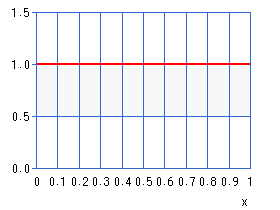
\includegraphics[width=\textwidth]{images/beta_1_1.png}
            \caption{$\alpha=1$, $\beta=1$}
            \label{sec:bhh:hyper_parameters:normalisation_beta_1_1}
      \end{subfigure}
      \begin{subfigure}{0.5\textwidth}
            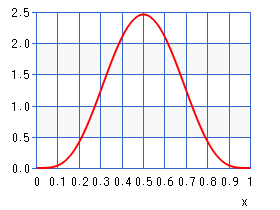
\includegraphics[width=\textwidth]{images/beta_5_5.png}
            \caption{$\alpha=5$, $\beta=5$}
            \label{sec:bhh:hyper_parameters:normalisation_beta_5_5}
      \end{subfigure}
      \par\bigskip
      \begin{subfigure}{0.5\textwidth}
            \centering
            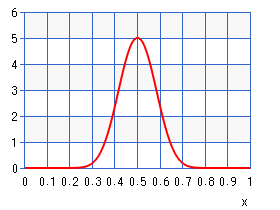
\includegraphics[width=\textwidth]{images/beta_20_20.png}
            \caption{$\alpha=20$, $\beta=20$}
            \label{sec:bhh:hyper_parameters:normalisation_beta_20_20}
      \end{subfigure}
      \par\bigskip
      \caption{Beta probability distribution with varying $\alpha$ and $\beta$ values.}
      \label{sec:bhh:hyper_parameters:discounted_rewards:normalisation}
\end{figure}

This concludes the hyper-parameters that are used by the \ac{BHH}. The following section discusses the default value for proxied update step operations.

\subsection{Defaults}
\label{sec:bhh:hyper_parameters:defaults}

Section \ref{sec:bhh:heuristic:proxies} provided the reader with the concept of proxied heuristic update step operations. As was mentioned in Section \ref{sec:bhh:hyper_parameters:heuristic_pool}, low-level heuristics each have their own set of hyper-parameters as well. This means that a set of default low-level parameters must be allocated specifically for these proxies. Consider a scenario where two instances of \ac{Adam} is included in the heuristic pool. Each has its own set of hyper-parameters that (should) differ from each other. In the case of \ac{Adam}, there are 4 hyper-parameters that include learning rate, $\beta1$, $\beta2$ and $\epsilon$. If another heuristic needs to proxy \ac{Adam}'s ``expected gradient mean operation'', a default $\beta1$ parameter must be supplied. Notice that this is only the case where multiple instances of a heuristic is included and there is uncertainty about which instance's hyper-parameters to use for the proxied heuristic update steps. If there is only one instance of a particular heuristic, that instance's hyper-parameters are used. The next section provides the reader with the pseudo-code algorithm for the \ac{BHH}.

\section{Algorithm}
\label{sec:bhh:algorithm}

This section provides the reader with a high level pseudo-code implementation of the \ac{BHH}. This is given in Algorithm \ref{algo:bhh} below.

\begin{algorithm}[H]
      \caption{The pseudo code for the \index{Bayesian Hyper-Heuristic} Bayesian Hyper-Heuristic optimiser}
      \label{algo:bhh}
      \begin{algorithmic}
            \State step $\gets 0$

            \State select initial heuristics
            \State initialise population and entities
            \State evaluate entities' initial position
            \State update population state

            \While{stopping condition not met}
            \For{all entities in entity pool}
            \If{selected heuristic is gradient-based}
            \State get gradients
            \EndIf

            \State apply low-level heuristic and proxy operations
            \State update population state
            \State log performance to performance log

            \If {step < burn-in window size}
            \State select heuristic
            \Else
            \If {step $\mathbin{\%}$ reanalysis window size = 0}
            \State apply Bayesian analysis
            \EndIf

            \If {step $\mathbin{\%}$ reselection window size = 0}
            \State select heuristic
            \EndIf

            \If {step > replay window size}
            \State prune performance log
            \EndIf
            \EndIf
            \EndFor
            \State step $\gets$ step + $1$
            \EndWhile
      \end{algorithmic}
\end{algorithm}

\section{Summary}
\label{sec:bhh:summary}

This chapter provided the reader with extensive detail on the inner workings and design of the \ac{BHH}. The \ac{BHH} was formally classified and the details around various components of the \ac{BHH}'s architecture was presented. Formal mathematical descriptions of the Bayesian selection method have been provided. The optimisation process, by means of Bayesian analysis has been presented and a pseudo code implementation of the \ac{BHH} was presented.

This concludes the background information and literature studies that is required to propose a methodology for an empirical process. This methodology is provided in the next chapter.
